\documentclass[tikz,border=10pt,multi=tikzpicture]{standalone}
\usepackage{amsmath}
\usepackage{xcolor}
\definecolor{mainblue}{HTML}{001158}
\definecolor{accent}{HTML}{8592bc}
\definecolor{lightaccent}{HTML}{e7e9f2}
\definecolor{loadcolor}{HTML}{e67e22}

\begin{document}

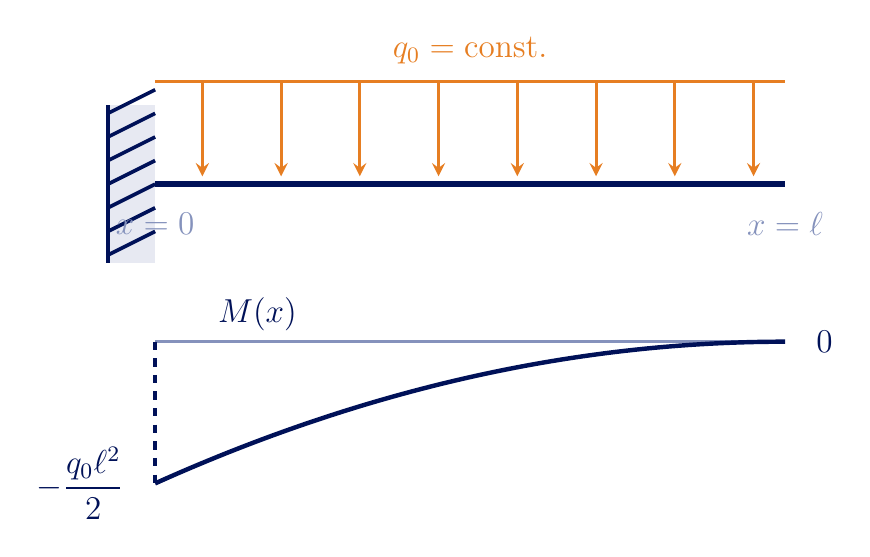
\begin{tikzpicture}[>=stealth, line width=1.3pt, font=\large]
  % wall / fixed support
  \fill[lightaccent] (-0.6,-1.0) rectangle (0,1.0);
  \foreach \y in {-0.9,-0.6,...,0.9} {
    \draw[mainblue] (-0.6,\y) -- (0,\y+0.3);
  }
  \draw[mainblue, line width=1.4pt] (-0.6,-1.0) -- (-0.6,1.0);

  % beam
  \draw[mainblue, line width=2pt] (0,0) -- (8,0);

  % distributed load q0 (uniform, downward arrows)
  \foreach \x in {0.6,1.6,...,7.6} {
    \draw[loadcolor, ->, line width=1.1pt] (\x,1.3) -- (\x,0.1);
  }
  \draw[loadcolor, line width=1.1pt] (0,1.3) -- (8,1.3);
  \node[loadcolor] at (4.0,1.7) {$q_0 = \text{const.}$};

  % coordinate x
  \node[accent] at (0,-0.5) {$x=0$};
  \node[accent] at (8,-0.5) {$x=\ell$};

  % moment diagram below (parabola: 0 at free end, -q0 l^2/2 at wall)
  \draw[accent] (0,-2.0) -- (8,-2.0);
  \draw[mainblue, line width=1.6pt] plot[domain=0:8,samples=60] (\x,{-2.0-1.8*((8-\x)/8)*((8-\x)/8)});
  \draw[mainblue, dashed] (0,-2.0) -- (0,-3.8);
  \node[mainblue] at (1.3,-1.65) {$M(x)$};
  \node[mainblue] at (-0.95,-3.8) {$-\dfrac{q_0\ell^2}{2}$};
  \node[mainblue] at (8.5,-2.0) {$0$};
\end{tikzpicture}

\end{document}
